%%%%%%%%%%%%%%%%%%%%%%%%%%%%%%%%%%%%%%%%%%%%%%%%%%%
%% LaTeX book template                           %%
%% Author:  XXX                                  %%
%%%%%%%%%%%%%%%%%%%%%%%%%%%%%%%%%%%%%%%%%%%%%%%%%%%

\documentclass[a4paper,11pt]{report}
\usepackage[T1]{fontenc}
\usepackage[utf8]{inputenc}
\usepackage{lmodern}
\usepackage{float}
%%%%%%%%%%%%%%%%%%%%%%%%%%%%%%%%%%%%%%%%%%%%%%%%%%%%%%%%%
% Source: http://en.wikibooks.org/wiki/LaTeX/Hyperlinks %
%%%%%%%%%%%%%%%%%%%%%%%%%%%%%%%%%%%%%%%%%%%%%%%%%%%%%%%%%
\usepackage{hyperref}
\usepackage[english]{babel}
\usepackage{graphicx}
\usepackage{caption}
\usepackage{subcaption}
\usepackage{listings}
\usepackage{fancybox}
\usepackage{minibox}
\usepackage{lipsum}
\usepackage{xcolor}






%%%%%%%%%%%%%%%%%%%%%%%%%%%%%%%%%%%%%%%%%%%%%%%%%%%
% First page of book which contains 'stuff' like: %
%  - Book title, subtitle                         %
%  - Book author name                             %
%%%%%%%%%%%%%%%%%%%%%%%%%%%%%%%%%%%%%%%%%%%%%%%%%%%

% Book's title and subtitle
\title{\Huge \textbf{A Guide on Zigbee}   \\ }
% Author
\author{\textsc{E-YANTRA Interns}\thanks{\url{www.eyantra.org}}}


\begin{document}

\maketitle


%%%%%%%%%%%%%%%%%%%%%%%%%%%%%%%%%%%%%%%%%%%%%%%%%%%%%%%%%%%%%%%%%%%%%%%%
% Auto-generated table of contents, list of figures and list of tables %
%%%%%%%%%%%%%%%%%%%%%%%%%%%%%%%%%%%%%%%%%%%%%%%%%%%%%%%%%%%%%%%%%%%%%%%%
\tableofcontents


%%%%%%%%%%%%%%%%
% NEW CHAPTER! %
%%%%%%%%%%%%%%%%
\chapter{Installation Steps For X-CTU}


\section{What is X-CTU?}
X-CTU is a Windows-based application provided by Digi. This program was designed to interact with the firmware files found on Digi’s RF products and to provide a simple-to-use graphical user interface to them. \vspace{5mm}  \\
\textbf{Software Requirement} \\
X-CTU is designed to function with all Windows-based computers running Microsoft Windows 98 SE and above.


\section{Steps for Installation.}
\subsection{\textbf{Step 1}}
Double click the “Setup\_XCTU\_5260.exe” in Software and Drivers folder provided in e-Yantra\_DVD. \\

\begin{figure}[H]
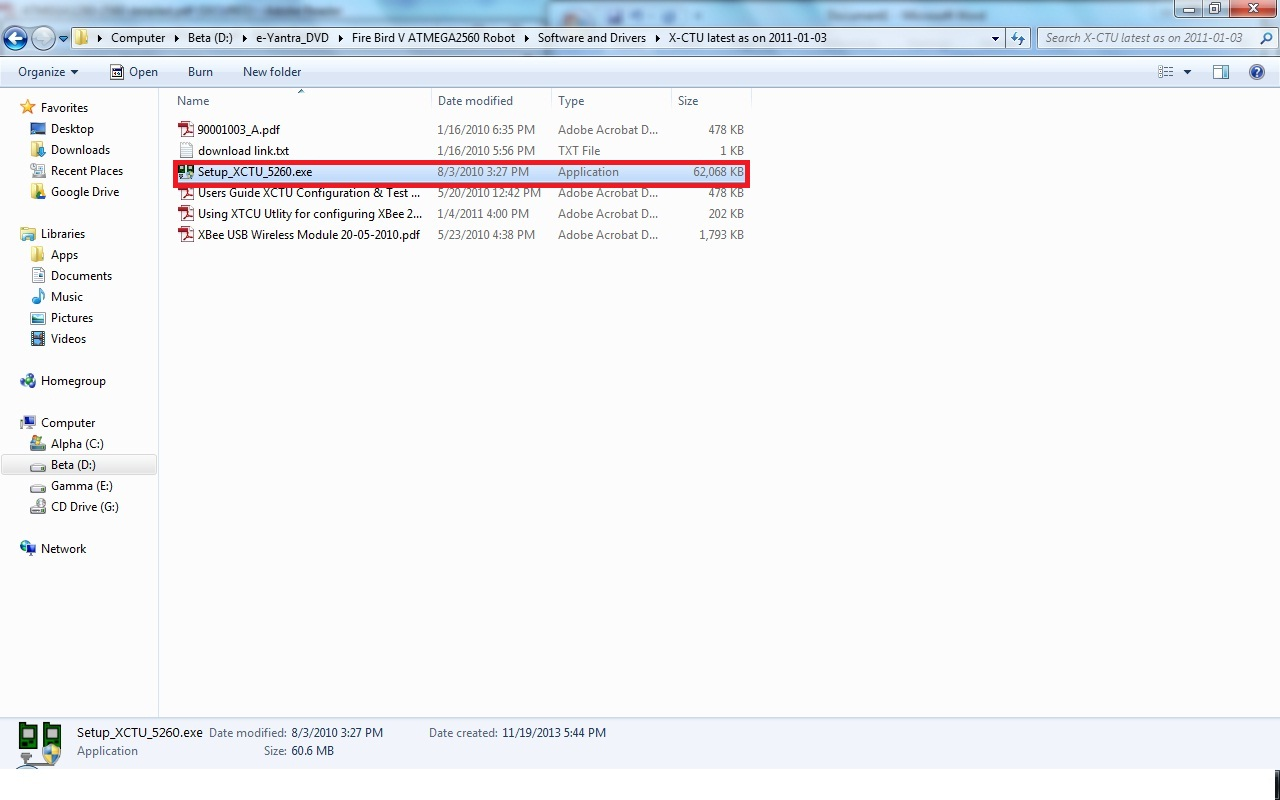
\includegraphics[width=1\linewidth]{SETUP_WINDOW}
\caption{Setup window}
\end{figure}

\subsection{\textbf{Step 2}}
Enter next as shown in figure.

\begin{figure}[H]
\centering
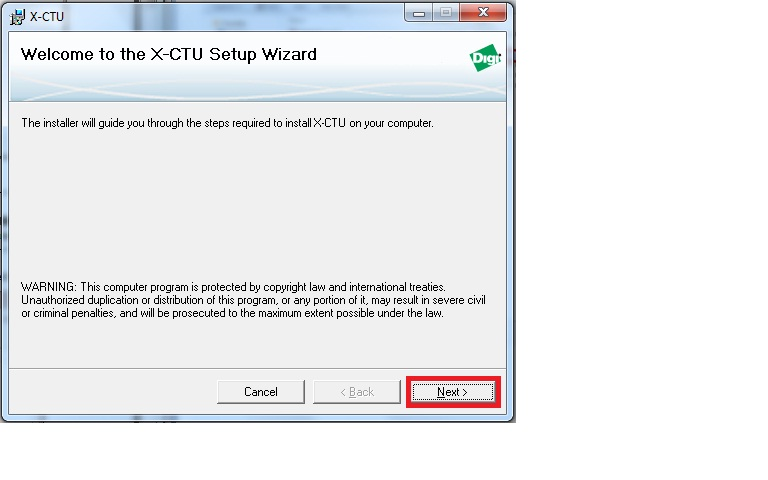
\includegraphics[width=1\linewidth]{Step2}
\caption{Press Next}
\end{figure}

\subsection{\textbf{Step 3}}
Select “I Agree” and press NEXT.

\begin{figure}[H]
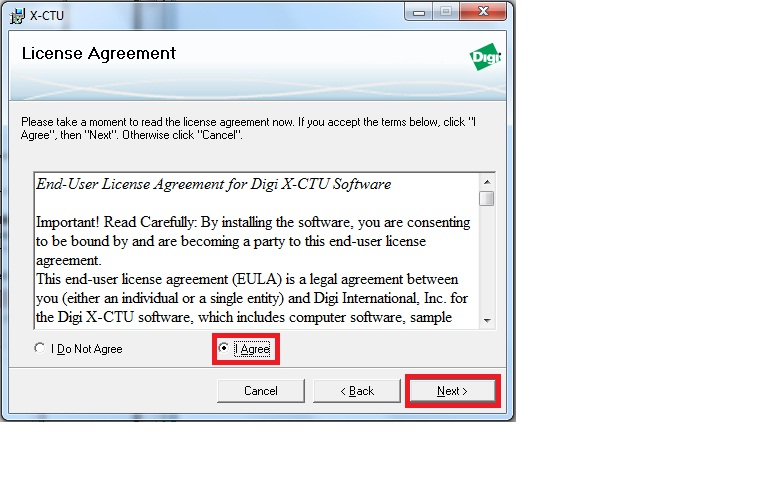
\includegraphics[width=1\linewidth]{Step3}
\caption{I Agree}
\end{figure}


\subsection{\textbf{Step 4}}
Select an installation folder and press NEXT.

\begin{figure}[H]
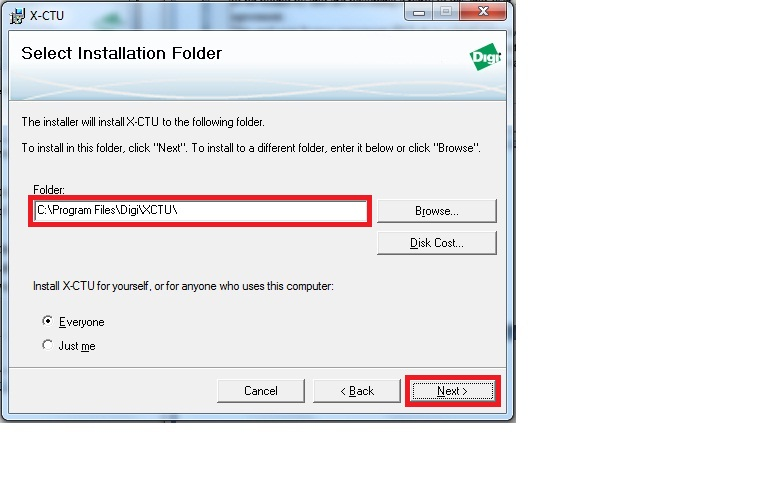
\includegraphics[width=1\linewidth]{Step4}
\caption{Installation Folder}
\end{figure}

\subsection{\textbf{Step 5}}
Click “NEXT” to start the installation.

\begin{figure}[H]
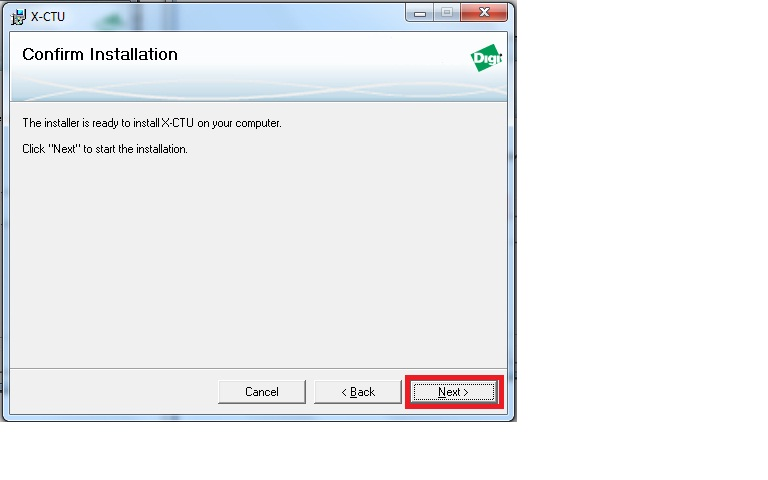
\includegraphics[width=1\linewidth]{Step5}
\caption{Start Installation}
\end{figure}


\subsection{\textbf{Step 6}}
The installation will take about five minutes to complete.

\begin{figure}[H]
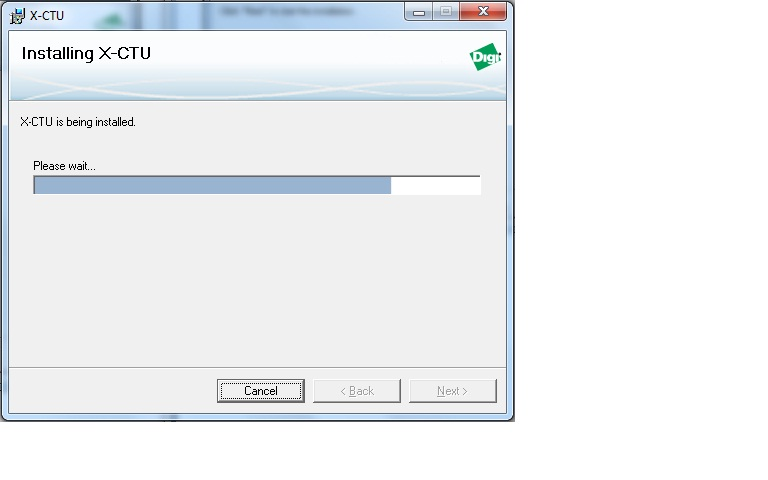
\includegraphics[width=1\linewidth]{Step6-A}
\caption{Installing window}
\end{figure}

You have now successfully installed X-CTU . Click “close” to exit.

\begin{figure}[H]
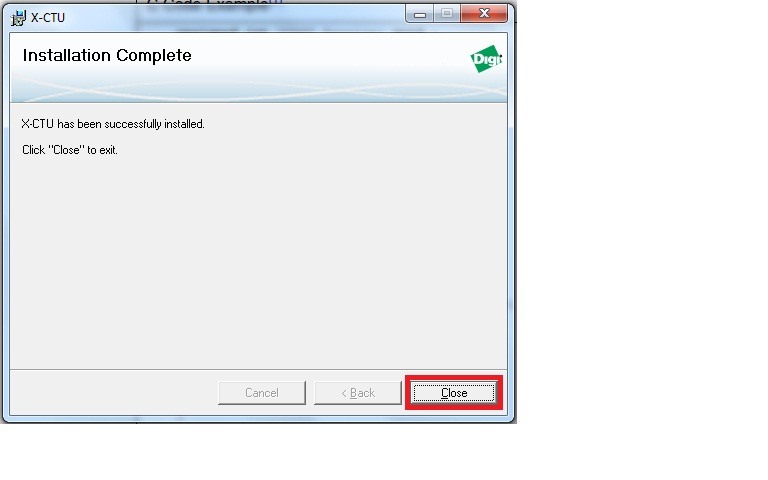
\includegraphics[width=0.9\linewidth]{Step6-B}
\caption{Close}
\end{figure}



\subsection{\textbf{Step 7}}
When properly installed it can be launched by clicking on the icon on the PC desktop  (see Figure 1)  or selecting from the Start menu  (see Figure 2).

\begin{figure}[H]
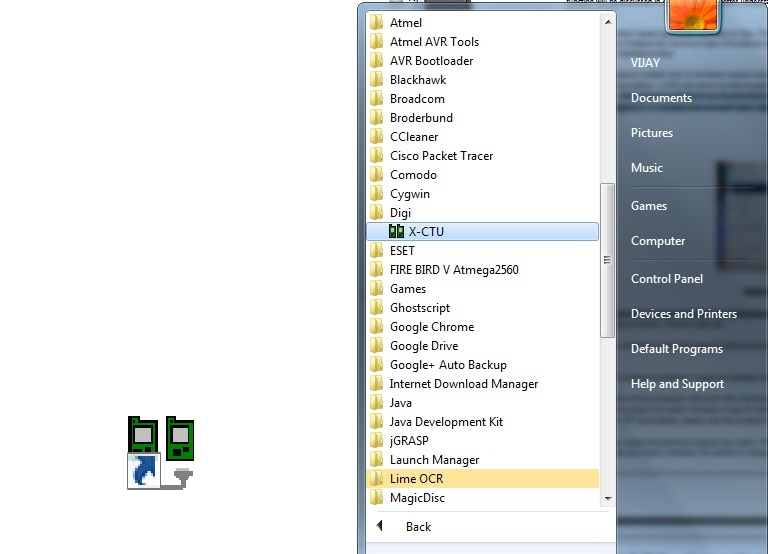
\includegraphics[width=1\linewidth]{finalstep}
\caption{Opening X-CTU}
\end{figure}


\chapter{Unicast Mode}
\section{Connecting the X-bee modules to the PC in Unicast mode}
\subsection{Step 1:Inserting XBEE in XBEE adaptor}
After Installation of the X-CTU software connection (which is clearly specified in installation guide of X-CTU ) . Now fix the X-bee module in the X-bee adapter which will help to connect the X-Bee with PC easily, Images clearly explain the fixing of X-Bee to the adapter. Placing it in opposite direction can damage the XBEE.
\begin{figure}[H]
\centering
\begin{subfigure}{.3\textwidth}
  \centering
  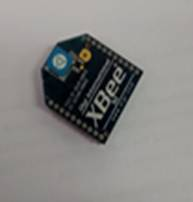
\includegraphics[width=1\linewidth]{image004}
  \caption{X-bee Module}
  \label{fig:sub1}
\end{subfigure}%
\begin{subfigure}{.3\textwidth}
  \centering
  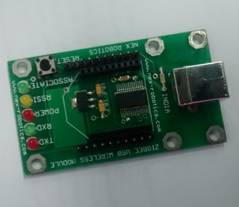
\includegraphics[width=1\linewidth]{image003}
  \caption{Xbee-Adaptor}
  \label{fig:sub2}
\end{subfigure}
\begin{subfigure}{.3\textwidth}
  \centering
  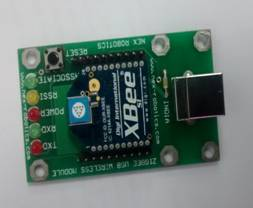
\includegraphics[width=1\linewidth]{image002}
  \caption{module in adaptor}
  \label{fig:sub2}
\end{subfigure}
\caption{Insterting X-Bee in adaptor}
\label{fig:test}
\end{figure}


\subsection{Step 2:Connecting XBEE module to PC.}
Make the connection between laptop and XBEE module using a USB cable as shown in figure.1.4.Once after the connection is established check for the power led(continuous on) and associate led(blink) in the adapter. If not remove and insert the USB and repeat the step 1
\begin{figure}[H]
\centering
\begin{subfigure}{.5\textwidth}
  \centering
  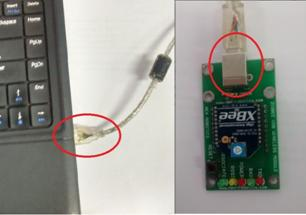
\includegraphics[width=1\linewidth]{image007}
  \caption{connection between pc and x-bee}
  \label{fig:sub1}
\end{subfigure}%
\begin{subfigure}{.5\textwidth}
  \centering
  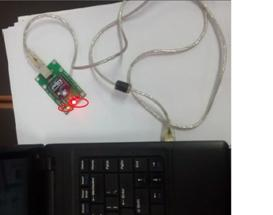
\includegraphics[width=1\linewidth]{image006}
  \caption{Xbee-Adaptor}
  \label{fig:sub2}
\end{subfigure}
\caption{Power and Associate LED }
\label{fig:test}
\end{figure}







\subsection{Step 3:Com port settings.}
After connecting X-bee to the PC, Now check whether the necessary com port is assigned to the X-bee this can be done in Device manager. If the com port is not assigned ,You will need to install driver for FT232 USB to serial converter.(Steps to install drives for FT232 USB to Serial Converter are covered in detail in the section 6.5 of the Hardware Manual)
\begin{figure}[H]
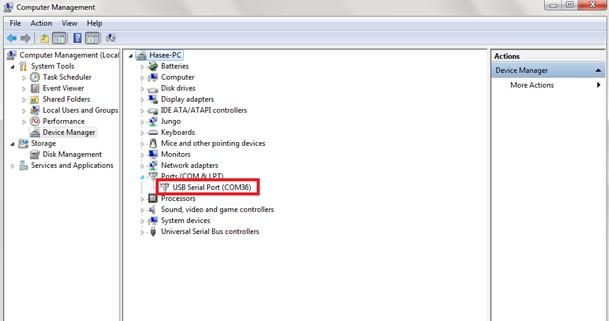
\includegraphics[width=1\linewidth]{image008}
\caption{Device manager}
\end{figure}


\subsection{Step4: Launching X-CTU Software.}
 Now open X-CTU application which you have installed earlier. This can be done in any of the two ways by selecting the icon from desktop or select it from the start menu
 \begin{figure}[H]
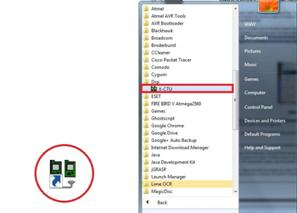
\includegraphics[width=1\linewidth]{image009}
\caption{X-CTU icon in desktop and in start menu }
\end{figure}


\subsection{Step5: X-CTU window}
After this X-CTU window will pop up as shown in the figure
 \begin{figure}[H]
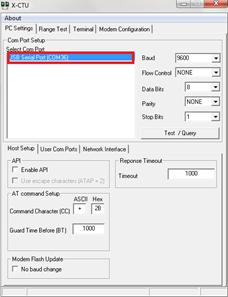
\includegraphics[width=1\linewidth]{image010}
\caption{X-CTU window }
\end{figure}


\subsection{Step6: Testing and Querying the Network by Serial number verification.}
 Now we need to read the serial number and the type of modem by clicking on the ‘Test/ Query’ button. Suddenly a window pops with the serial number and type of the modem.
 \begin{figure}[H]
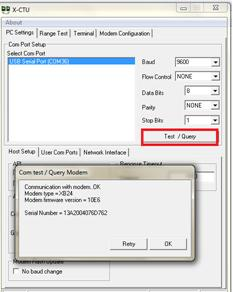
\includegraphics[width=1\linewidth]{image011}
\caption{Com test/Query modem }
\end{figure}

Once this window pops its fine to work, detailed explanation and function 
about X-CTU’s various tab is given in e-Yantra\_DVD\textbackslash Fire Bird V 
ATMEGA2560 Robot\textbackslash Accessories\textbackslash XBee USB Wireless Module\textbackslash Users Guide X-
CTU Configuration \& Test Utility Software \\

\framebox(315,215){%
    \parbox{300\unitlength}{\textbf{UNICAST MODE} : In unicast mode there is data transfer from one server to end user and this is a bidirectional data transfer from server to end user and vice versa. Unicast is otherwise called as peer to peer communication. There are two ways of transmitting in unicast
    \begin{itemize}
    \item 16bit address mode
    \item 64bit address mode
    \end{itemize}
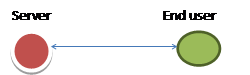
\includegraphics[width=1\linewidth]{image012}
}%
}


\subsection{Step8: Launching two X-CTUs}
Open two instances of X-CTU, in that select the required com port in each X-CTU so that one may act as the server and the other may act as the end user.

\begin{figure}[H]
\centering
\begin{subfigure}{.5\textwidth}
  \centering
  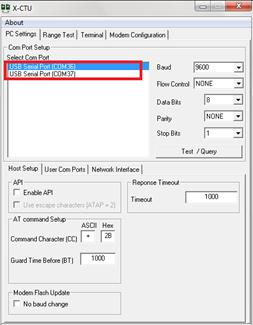
\includegraphics[width=1\linewidth]{image016}
  \label{fig:sub1}
\end{subfigure}%
\begin{subfigure}{.5\textwidth}
  \centering
  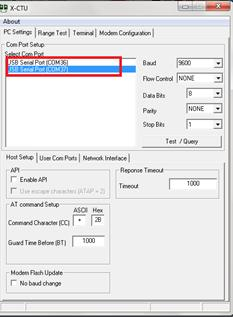
\includegraphics[width=1\linewidth]{image015}
  \label{fig:sub1}
\end{subfigure}%
\caption{X-CTU with different ports selected }
\label{fig:test}
\end{figure}
 
\subsection{Step9: Testing and Querying with serial number check.}
Check for the unique serial id from the X-bee by clicking on the test and query button \\ \\
\framebox(355,85){%
    \parbox{350\unitlength}{\textbf{Serial Number} :\\ A unique 64-bit IEEE source address is assigned at the factory and can be read with the SL (Serial Number Low) and SH (Serial Number High) commands. Short addressing must be configured manually. A module will use its unique 64-bit address as its Source Address if it’s MY (16-bit Source Address) value is “0xFFFF” or “0xFFFE”.
}%
}

\begin{figure}[H]
\centering
\begin{subfigure}{.5\textwidth}
  \centering
  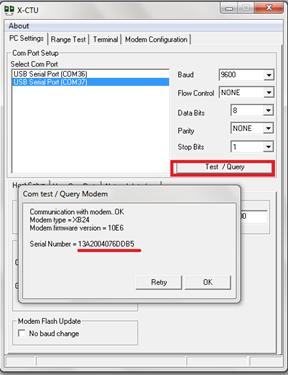
\includegraphics[width=1\linewidth]{image019}
  \label{fig:sub1}
\end{subfigure}%
\begin{subfigure}{.5\textwidth}
  \centering
  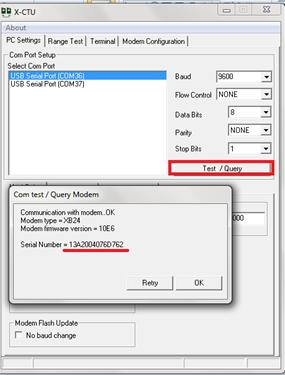
\includegraphics[width=1\linewidth]{image017}
  \label{fig:sub1}
\end{subfigure}%
\caption{X-bee with different serial number}
\label{fig:test}
\end{figure}


\subsection{Step10: Reading the module}
Open modem configuration tab on the X-CTU window and read the modem.
\begin{figure}[H]
\centering
\begin{subfigure}{.5\textwidth}
  \centering
  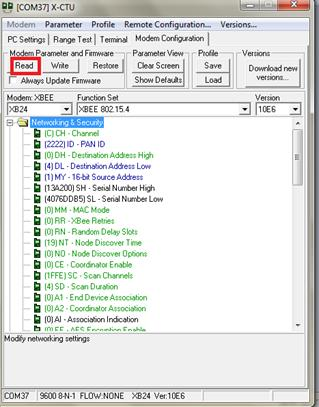
\includegraphics[width=1\linewidth]{image021}
  \label{fig:sub1}
\end{subfigure}%
\begin{subfigure}{.5\textwidth}
  \centering
  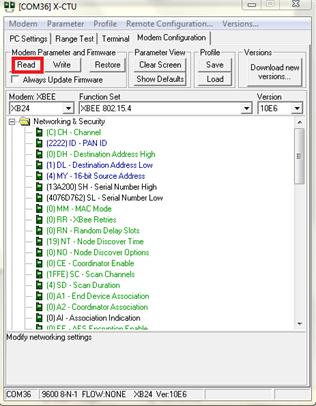
\includegraphics[width=1\linewidth]{image020}
  \label{fig:sub1}
\end{subfigure}%
\caption{Reading existing configuration}
\label{fig:test}
\end{figure}

The X-CTU will read the pre-configuration of XBEE.

\subsection{Step11: Setting the network address}

Now click on the modem configuration on the top of the window to configure the various address location and pan id. \\

In this case unicast 16 bit mode :
\begin{itemize}
\item Make the PAN ID same for both server and end user because they should be in the same network for communication
\item Make the destination address of server as the source address of end user. 	
\item Make the destination address of end user as the source address of server. 	
\end{itemize}
In case of unicast 64 bit mode:
\begin{itemize}
\item Make all PAN ID same.
\item Make the destination of server with the serial number of the end user and source as FFFE.
\item Make the destination of end user with the serial number of the server and source as FFFE. 	
\end{itemize}

\begin{figure}[H]
\centering
  \centering
  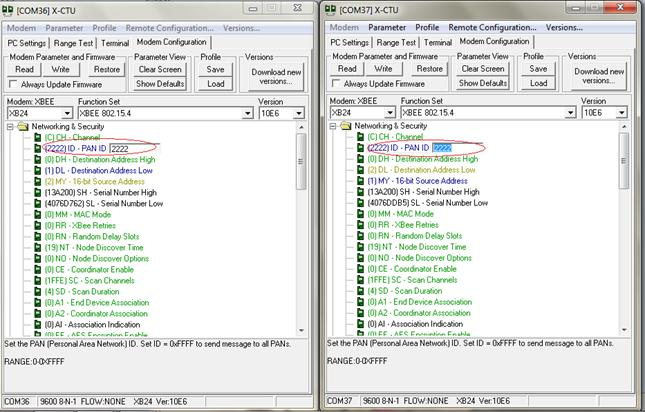
\includegraphics[width=1\linewidth]{image024}
  \label{fig:sub1}
\caption{Making the PAN ID same}
\label{fig:test}
\end{figure}

\begin{figure}[H]
\centering
  \centering
  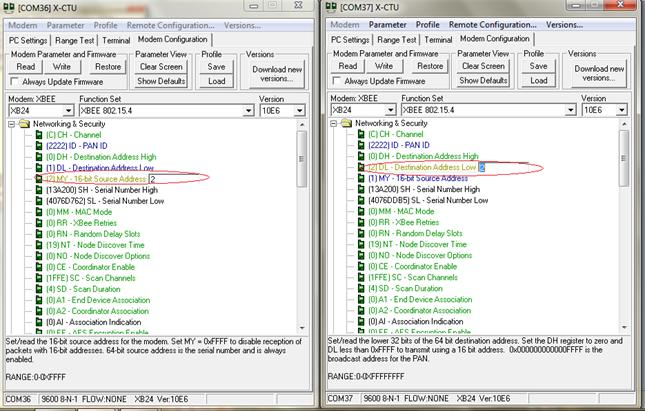
\includegraphics[width=1\linewidth]{image025}
  \label{fig:sub1}
\caption{make source address of server same as the destination address of end}
\label{fig:test}
\end{figure}

\begin{figure}[H]
\centering
  \centering
  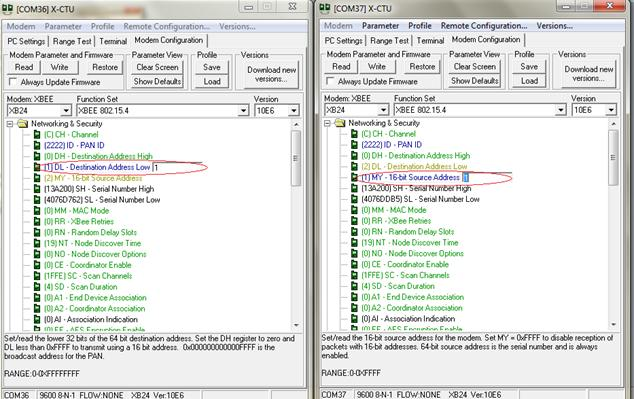
\includegraphics[width=1\linewidth]{image026}
  \label{fig:sub1}
\caption{make source address of server same as the destination address of end }
\label{fig:test}
\end{figure}

\begin{figure}[H]
\centering
  \centering
  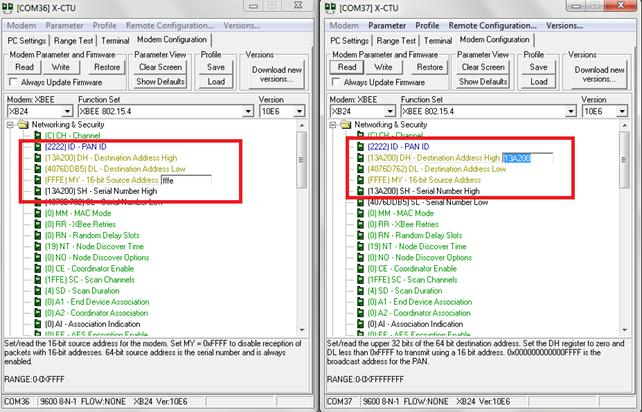
\includegraphics[width=1\linewidth]{image029}
  \label{fig:sub1}
\caption{64-bit addressing mode.}
\label{fig:test}
\end{figure}

\framebox(315,595){%
    \parbox{300\unitlength}{\textbf{Key Terms} : 
    \begin{itemize}
    \item \textbf{Channel(CH): }802.15.4 and Zigbee break the 2.4Ghz band into 16 channels. Parameter range for Xbee is 0x0B - 0x1A.
    \item \textbf{Personal Area Network(PAN):}A data communication network that includes one or more End Devices and optionally a Coordinator.
    \item \textbf{PAN ID:}  Each network is defined with a unique PAN identifier (PAN ID). This identifier is common among all devices of the same network.  ZigBee devices are either preconfigured with a PAN ID to join, or they can discovery nearby networks and select a PAN ID to join.
If multiple Zigbee networks are operating within range of each other, each should have unique PAN ID.
	
	\item \textbf{Destination Address:}
		\begin{itemize}
		\item \textbf{DH:} Destination Address High. Set/Read the upper 32 bits of the 64-bit destination address. When combined with DL, it defines the destination address used for transmission. To transmit using a 16-bit address, set DH parameter to zero and DL less than 0xFFFF. 0x000000000000FFFF is the broadcast address for the PAN.
		\item \textbf{DL:} Destination Address Low. Set/Read the lower 32 bits of the 64-bit destination address. When combined with DH, DL defines the destination address used for transmission. To transmit using a 16-bit address, set DH parameter to zero and DL less than 0xFFFF. 0x000000000000FFFF is the broadcast address for the PAN.
		\end{itemize}
	\item \textbf{Source Address:}
		\item \textbf{16-bit (MY):} Set/Read the RF module 16-bit source address. Set MY = 0xFFFF to disable reception of packets with 16-bit addresses
		\item \textbf{64-bit (MY):} 64-bit source address (serial number) and broadcast address (0x000000000000FFFF) is always enabled.
\end{itemize}
}%
}
\newpage
\framebox(315,135){%
    \parbox{300\unitlength}{
			\begin{itemize}
			\item \textbf{	SH: Serial Number High.} Read high 32 bits of the RF module's unique IEEE 64-bit address. 64-bit source address is always enabled.
			\item \textbf{	 SL: Serial Number Low.} SL: Serial Number Low. Read low 32 bits of the RF module's unique IEEE 64-bit address. 64-bit source address is always enabled.
			\end{itemize}
}%
}

\subsection{Step12: Writing the module}
Write this configuration into the module by clicking on write option.
\begin{figure}[H]
\centering
\begin{subfigure}{.5\textwidth}
  \centering
  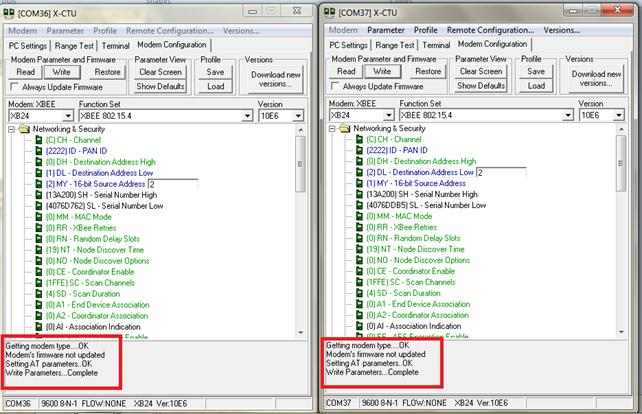
\includegraphics[width=1\linewidth]{image030}
  \label{fig:sub1}
\end{subfigure}%
\caption{Writing the module}
\label{fig:test}
\end{figure}


\subsection{Step13: Verification of Unicast Network Configuration}
Now to see the output open the terminal window in both X-CTU. Type something in window which gets reflected back in other. The transmitted data will appear in blue while the received data appear in red
\begin{figure}[H]
\centering
\begin{subfigure}{.5\textwidth}
  \centering
  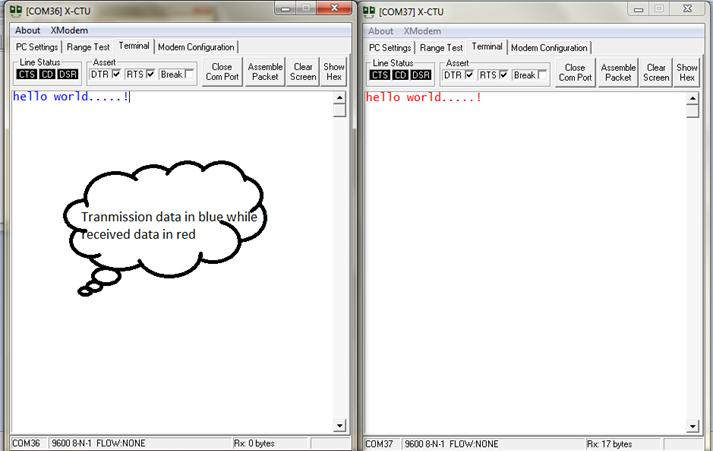
\includegraphics[width=1\linewidth]{image032}
  \label{fig:sub1}
\end{subfigure}%
\caption{Terminal Window}
\label{fig:test}
\end{figure}

\begin{figure}[H]
\centering
\begin{subfigure}{.5\textwidth}
  \centering
  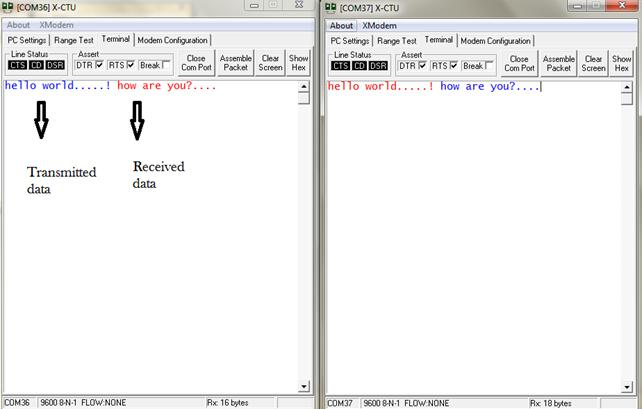
\includegraphics[width=1\linewidth]{image033}
  \label{fig:sub1}
\end{subfigure}%
\caption{Terminal Window}
\label{fig:tab}
\end{figure}
\subsection{conclusion}
\framebox(315,205){%
    \parbox{300\unitlength}{\textbf{Conclusion} : \\
    As it is as shown in \ref{fig:tab} :
    \begin{itemize}
    \item [com36] is server [com37] is end user.\dots
    \item Data transmitted by server is received at end user and data transmitted by end users are only received by the server. \dots
    \item Message “hello world!.....” was sent by server [com36] and is received at the end users [com37]. Message “how are you?....” was sent by the end user [com37] and is received at the server [com36].\dots
    \item This is called ‘Unicast’. \dots
    \end{itemize}
}%
}
\newpage

\chapter{Broadcast}
\section{What is Broadcast?}
\textbf{Broadcast:} \\
\begin{figure}[H]
\centering
  \centering
  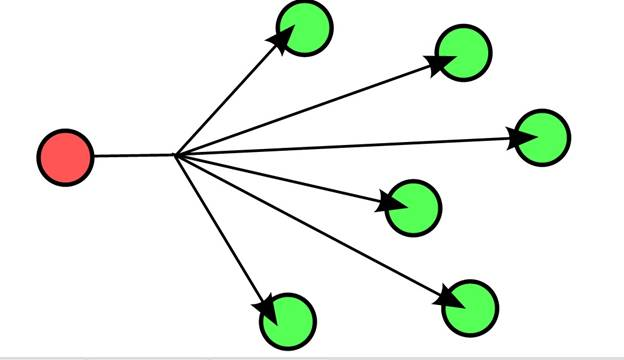
\includegraphics[width=1.2\linewidth]{bimage001}
  \label{fig:sub1}
\caption{Block Diagram}
\label{fig:test}
\end{figure}
The Broadcast Consists of a server who can communicate with his end users and the end users can communicate with the server but the end users cannot between themselves.
\section{Steps to configuring Broadcast}
The steps to create a Broadcast communication in XBEE module using 16-bit addressing are as follows:
\subsection{Step 1: Connecting Zigbee to PC.}
Make the connection between laptop and XBEE module using a USB cable as shown in figure.
\begin{figure}[H]
\centering
  \centering
  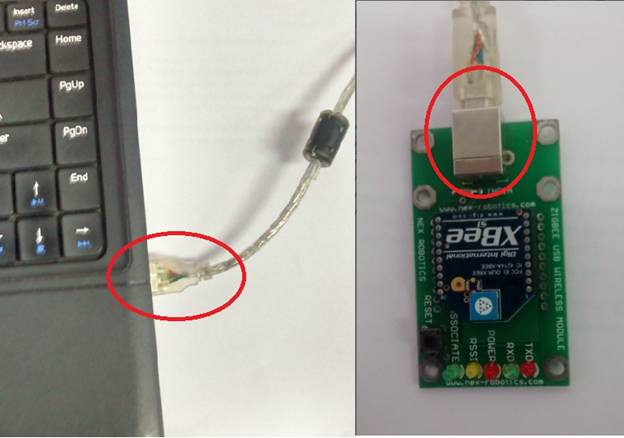
\includegraphics[width=1\linewidth]{bimage002}
  \label{fig:sub1}
\caption{USB connections}
\label{fig:test}
\end{figure}
The red Power LED in XBEE module must ON and green associate LED must start blinking.
\begin{figure}[H]
\centering
  \centering
  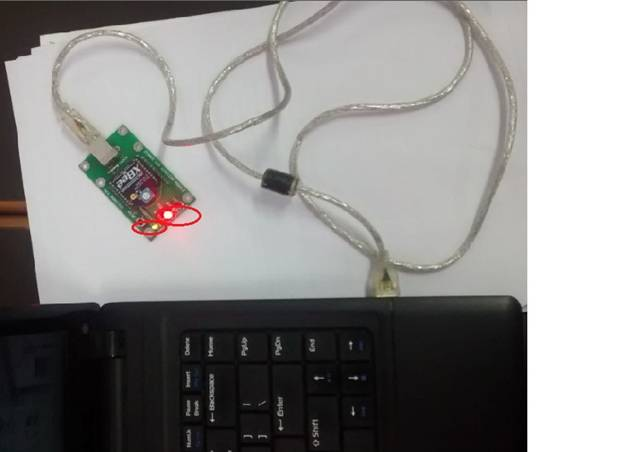
\includegraphics[width=1\linewidth]{bimage003}
  \label{fig:sub1}
\caption{Verification through LEDs}
\label{fig:test}
\end{figure}
Repeat the step 1 four times for four different modules.
\subsection{Step 2: Launching X-CTU Software.}
Launch X-CTU windows from shortcut icon on desktop or program files in start menu.
\begin{figure}[H]
\centering
  \centering
  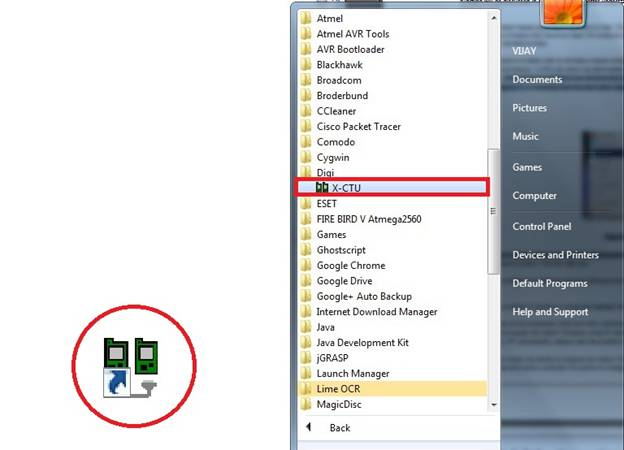
\includegraphics[width=1\linewidth]{bimage004}
  \label{fig:sub1}
\caption{Launching of X-CTU}
\label{fig:test}
\end{figure}
Do this for all four modules. Open multiple windows in same computer, one window for each module separately.

\subsection{Step 3: Testing and Querying the Network by Serial number verification.}
Notice the COM ports being displayed on the select COM port workspace. Test/Query each COM port individually in the windows opened previously. \\
	The result of Test/Query must show serial numbers as shown in figure 2 if the connections are correct.

\begin{figure}[H]
\centering
  \centering
  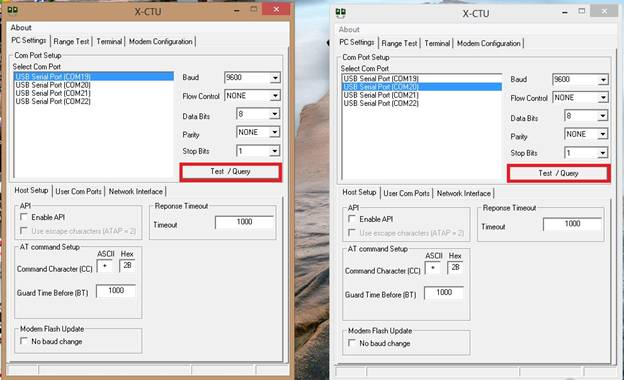
\includegraphics[width=1\linewidth]{bimage005}
  \label{fig:sub1}
\end{figure}
\begin{figure}[H]
\centering
  \centering
  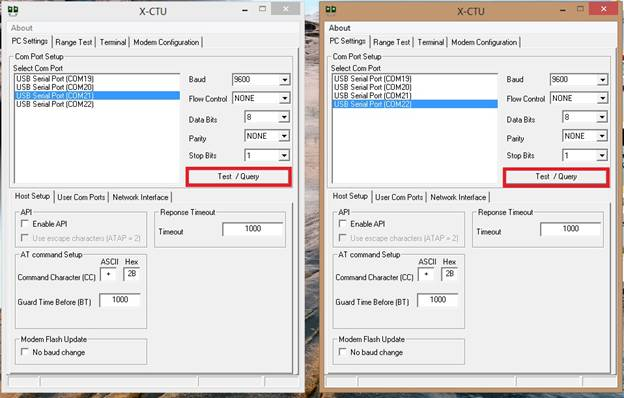
\includegraphics[width=1\linewidth]{bimage006}
  \label{fig:sub1}
\caption{ Test/Query}
\label{fig:test}
\end{figure}
\begin{figure}[H]
\centering
  \centering
  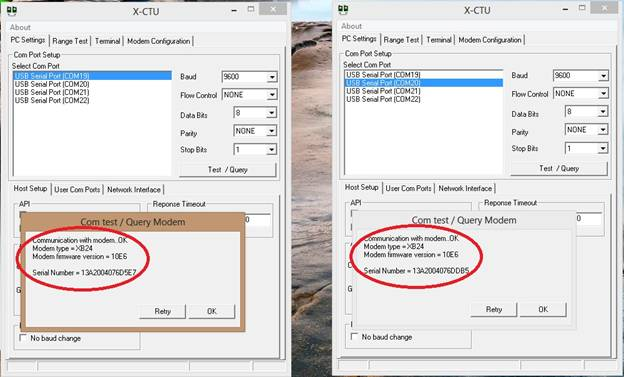
\includegraphics[width=1\linewidth]{bimage007}
  \label{fig:sub1}
\end{figure}
\begin{figure}[H]
\centering
  \centering
  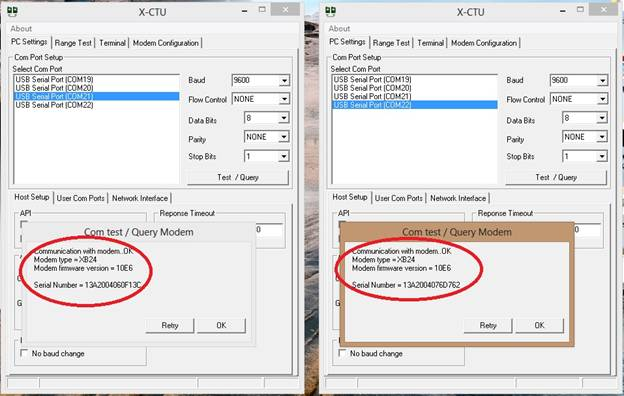
\includegraphics[width=1\linewidth]{bimage008}
  \label{fig:sub1}
\caption{serial number verification}
\label{fig:test}
\end{figure}
The above figures are for two windows, whereas you’ll have to do it for four windows .One window of one module each.

\subsection{Step 4: Reading the module.}
Open modem configuration tab on the X-CTU window and read the modem.

\begin{figure}[H]
\centering
  \centering
  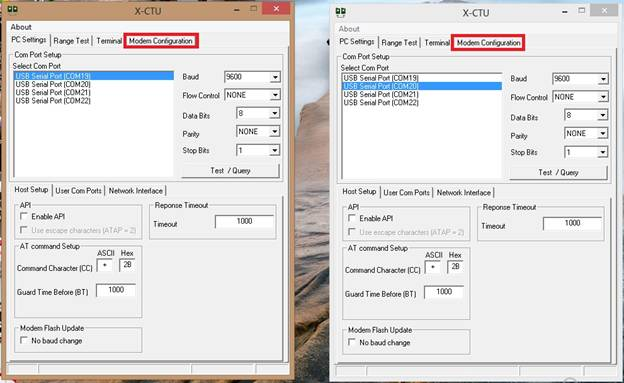
\includegraphics[width=1\linewidth]{bimage009}
  \label{fig:sub1}
\end{figure}
\begin{figure}[H]
\centering
  \centering
  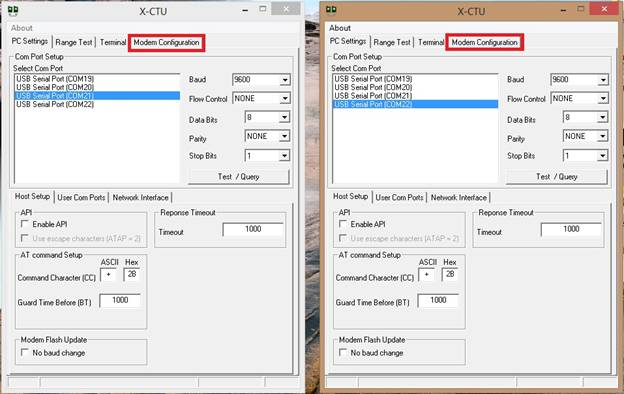
\includegraphics[width=1\linewidth]{bimage010}
  \label{fig:sub1}
\caption{ Modem Configuration}
\label{fig:test}
\end{figure}
\begin{figure}[H]
\centering
  \centering
  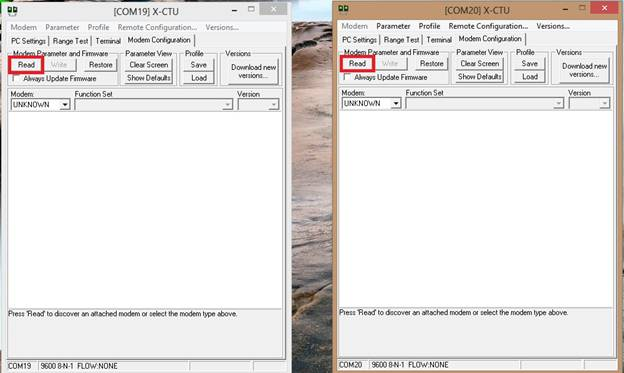
\includegraphics[width=1\linewidth]{bimage011}
  \label{fig:sub1}
\end{figure}
\begin{figure}[H]
\centering
  \centering
  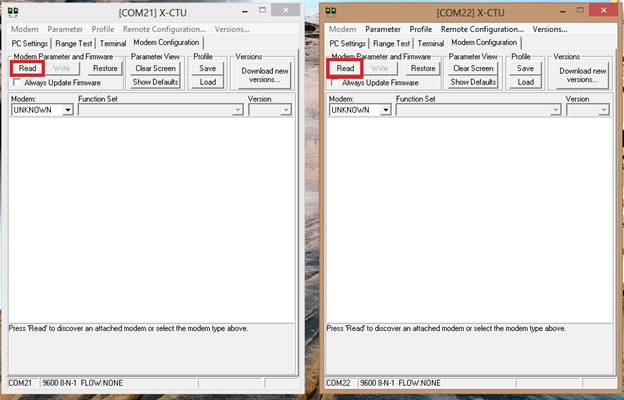
\includegraphics[width=1\linewidth]{bimage012}
  \label{fig:sub1}
\caption{Reading the module}
\label{fig:test}
\end{figure}
The X-CTU will read the pre-configuration of XBEE.


\subsection{Step 5: Setting the Network Address.}
In the workspace under Network \& Security tab select following settings

\begin{table}[ht]
\caption{X-CTU configuration} % title of Table
\centering % used for centering table
\begin{tabular}{|c|c|c|c|}
% centered columns (4 columns)
\hline\hline %inserts double horizontal lines
X-CTU(window 1) & X-CTU(window 2) & X-CTU(window 3) & X-CTU(window 3) \\ [0.5ex]
% inserts table
%heading
\hline % inserts single horizontal line
CH-Channel = C & CH-Channel = C & CH-Channel = C & CH-Channel = C \\
\hline
PAN ID = 2222 & PAN ID = 2222 & PAN ID = 2222 & PAN ID = 2222 \\
\hline
DH = 0 & DH = 0 & DH = 0 & DH = 0 \\
\hline
DL = FFFF & DL = 2 & DL = 2 & DL = 2 \\
\hline
MY = 2 & MY = 2 & MY = 2 & MY = 2 \\ [1ex] % [1ex] adds vertical space
\hline %inserts single line
\end{tabular}
\label{table:nonlin} % is used to refer this table in the text
\end{table}
\footnote{*this is a sample address and can be varied.}
\begin{itemize}
\item PAN IDs and Channel (CH) of all end users and server must same since they are operating in same network.
\item Since we are using 16-bit addressing mode DH of all modules must be 0.
\item DL of server should be broadcast address i.e. 0xFFFF.
\item DL of end user should be MY (source address) of server if you want end user to communicate back with server else it can be unique.
\item MY (source address) of end users should be unique since it should not be able to communicate with themselves. 

\end{itemize}


\framebox(315,155){%
    \parbox{300\unitlength}{\textbf{Key Terms} : 
    \begin{itemize}
    \item \textbf{Channel(CH): }802.15.4 and Zigbee break the 2.4Ghz band into 16 channels. Parameter range for Xbee is 0x0B - 0x1A.
    \item \textbf{Personal Area Network(PAN):}A data communication network that includes one or more End Devices and optionally a Coordinator.
    \end{itemize}
}%
}
\newpage
\framebox(315,575){%
    \parbox{300\unitlength}{
    \begin{itemize}
    \item \textbf{PAN ID:}  Each network is defined with a unique PAN identifier (PAN ID). This identifier is common among all devices of the same network.  ZigBee devices are either preconfigured with a PAN ID to join, or they can discovery nearby networks and select a PAN ID to join.
If multiple Zigbee networks are operating within range of each other, each should have unique PAN ID.
	
	\item \textbf{Destination Address:}
		\begin{itemize}
		\item \textbf{DH:} Destination Address High. Set/Read the upper 32 bits of the 64-bit destination address. When combined with DL, it defines the destination address used for transmission. To transmit using a 16-bit address, set DH parameter to zero and DL less than 0xFFFF. 0x000000000000FFFF is the broadcast address for the PAN.
		\item \textbf{DL:} Destination Address Low. Set/Read the lower 32 bits of the 64-bit destination address. When combined with DH, DL defines the destination address used for transmission. To transmit using a 16-bit address, set DH parameter to zero and DL less than 0xFFFF. 0x000000000000FFFF is the broadcast address for the PAN.
		\end{itemize}
	\item \textbf{Source Address:}
		\begin{itemize}
		\item \textbf{16-bit (MY):} Set/Read the RF module 16-bit source address. Set MY = 0xFFFF to disable reception of packets with 16-bit addresses
		\item \textbf{64-bit (MY):} 64-bit source address (serial number) and broadcast address (0x000000000000FFFF) is always enabled.
			\begin{itemize}
			\item \textbf{	SH: Serial Number High.} Read high 32 bits of the RF module's unique IEEE 64-bit address. 64-bit source address is always enabled.
			\item \textbf{	 SL: Serial Number Low.} SL: Serial Number Low. Read low 32 bits of the RF module's unique IEEE 64-bit address. 64-bit source address is always enabled.
			\end{itemize}
		\end{itemize}
	

    
    \end{itemize}
}%
}

\begin{figure}[H]
\centering
  \centering
  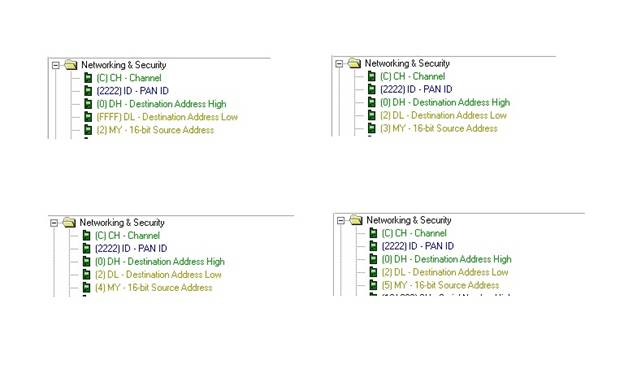
\includegraphics[width=1\linewidth]{bimage013}
  \caption{Network addressing}
  \label{fig:sub1}
\end{figure}

\subsection{Step 6:Writing the module}
Write this configuration to the module by clicking write option.
\begin{figure}[H]
\centering
  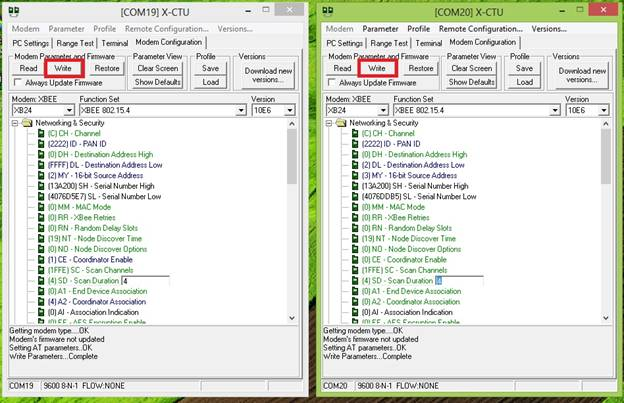
\includegraphics[width=1\linewidth]{bimage014}
  \label{fig:sub1}
\end{figure}

\begin{figure}[H]
\centering
  \centering
  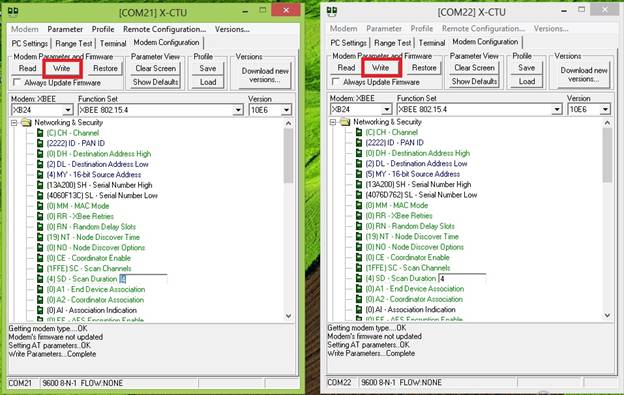
\includegraphics[width=1\linewidth]{bimage015}
  \caption{Writing the module}
  \label{fig:sub1}
\end{figure}

\subsection{Step 7: Verification of Broadcast Network Configuration.}
Go to terminal window and check if the transmission is a valid.\\
	In Terminal Window you can transmit by typing in the workspace.
	
	
	\begin{figure}[H]
\centering
  \centering
  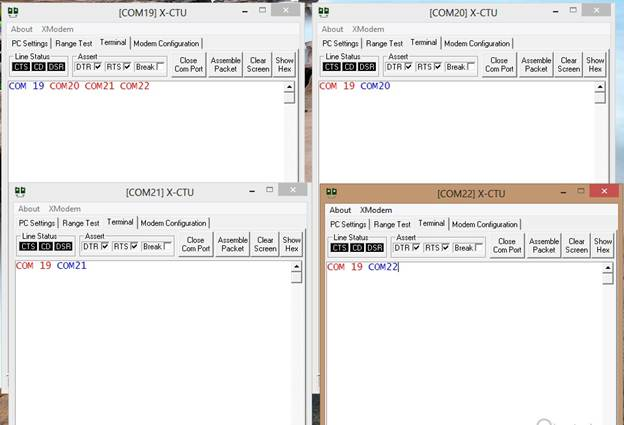
\includegraphics[width=1\linewidth]{bimage016}
  \caption{verification of Broadcast from terminal window}
  \label{fig:sag}
\end{figure}
\footnote{In above fig. blue letters are data written to be transmitted, while red letters are data received.}
\subsection{conclusion}
\framebox(325,170){%
    \parbox{300\unitlength}{\textbf{Conclusion} : \\
    As it is as shown in \ref{fig:sag} :
    \begin{itemize}
    \item [com19] is server and [com20][com21][com22] are end user. \dots
\item Data sent by server is received at all end user and data transmitted by end users are only received by server. \dots
\item Message “com19” was sent by server and is received by all receivers. Message “com20” “com21” “com22” was sent by end users and received only by server \dots
\item This is called ‘Broadcasting’.\dots

    \end{itemize}
}%
}
\newpage



\chapter{Multicast}
\section{What is Multicast?}
\textbf{Multicast:} \\
\begin{figure}[H]
\centering
  \centering
  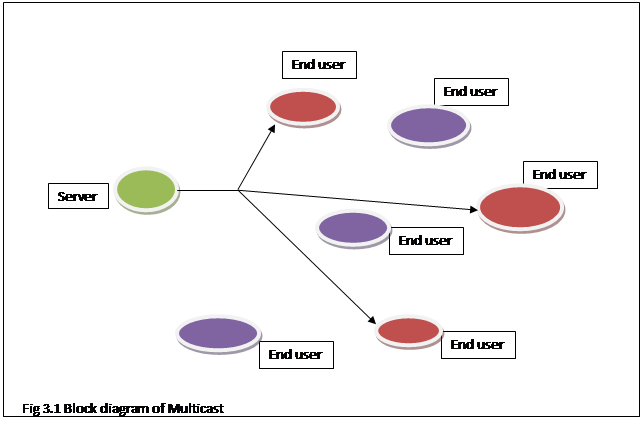
\includegraphics[width=1.2\linewidth]{mimage001}
  \label{fig:sub1}
\caption{Block Diagram}
\label{fig:test}
\end{figure}
The Multicast Consists of a server who can communicate with selected end users and these end users can communicate with the server but the end users cannot between themselves and end users not connected to server are totally not in connection with either server or selected end users.
\section{Steps to configuring Multicast}
The steps to create a multicast communication in XBEE module using 16-bit addressing are as follows:
\subsection{Step 1: Connecting Zigbee to PC.}
Make the connection between laptop and XBEE module using a USB cable as shown in figure.
\begin{figure}[H]
\centering
  \centering
  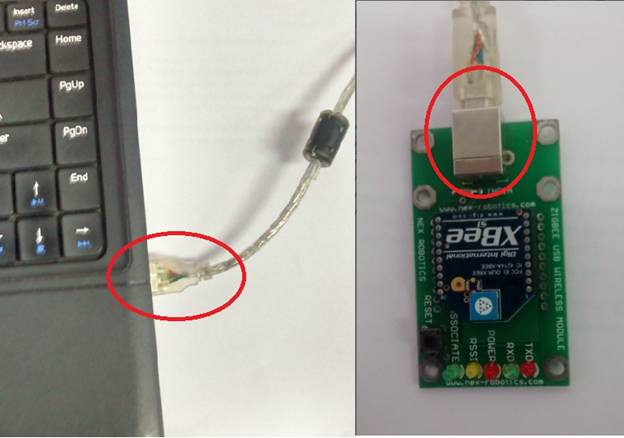
\includegraphics[width=1\linewidth]{bimage002}
  \label{fig:sub1}
\caption{USB connections}
\label{fig:test}
\end{figure}
The red Power LED in XBEE module must ON and green associate LED must start blinking.
\begin{figure}[H]
\centering
  \centering
  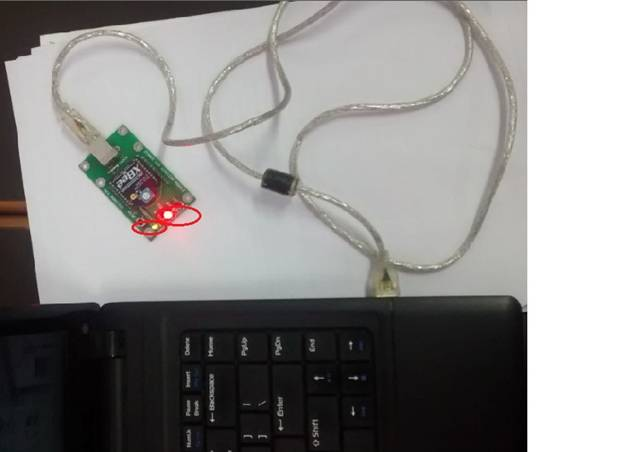
\includegraphics[width=1\linewidth]{bimage003}
  \label{fig:sub1}
\caption{Verification through LEDs}
\label{fig:test}
\end{figure}
Repeat the step 1 four times for four different modules.
\subsection{Step 2: Launching X-CTU Software.}
Launch X-CTU windows from shortcut icon on desktop or program files in start menu.
\begin{figure}[H]
\centering
  \centering
  \includegraphics[width=1\linewidth]{bimage004}
  \label{fig:sub1}
\caption{Launching of X-CTU}
\label{fig:test}
\end{figure}
Do this for all four modules. Open multiple windows in same computer, one window for each module separately.

\subsection{Step 3: Testing and Querying the Network by Serial number verification.}
Notice the COM ports being displayed on the select COM port workspace. Test/Query each COM port individually in the windows opened previously. \\
	The result of Test/Query must show serial numbers as shown in figure 2 if the connections are correct.

\begin{figure}[H]
\centering
  \centering
  \includegraphics[width=1\linewidth]{bimage005}
  \label{fig:sub1}
\end{figure}
\begin{figure}[H]
\centering
  \centering
  \includegraphics[width=1\linewidth]{bimage006}
  \label{fig:sub1}
\caption{ Test/Query}
\label{fig:test}
\end{figure}
\begin{figure}[H]
\centering
  \centering
  \includegraphics[width=1\linewidth]{bimage007}
  \label{fig:sub1}
\end{figure}
\begin{figure}[H]
\centering
  \centering
  \includegraphics[width=1\linewidth]{bimage008}
  \label{fig:sub1}
\caption{serial number verification}
\label{fig:test}
\end{figure}
The above figures are for two windows, whereas you’ll have to do it for four windows .One window of one module each.

\subsection{Step 4: Reading the module.}
Open modem configuration tab on the X-CTU window and read the modem.

\begin{figure}[H]
\centering
  \centering
  \includegraphics[width=1\linewidth]{bimage009}
  \label{fig:sub1}
\end{figure}
\begin{figure}[H]
\centering
  \centering
  \includegraphics[width=1\linewidth]{bimage010}
  \label{fig:sub1}
\caption{ Modem Configuration}
\label{fig:test}
\end{figure}
\begin{figure}[H]
\centering
  \centering
  \includegraphics[width=1\linewidth]{bimage011}
  \label{fig:sub1}
\end{figure}
\begin{figure}[H]
\centering
  \centering
  \includegraphics[width=1\linewidth]{bimage012}
  \label{fig:sub1}
\caption{Reading the module}
\label{fig:test}
\end{figure}
The X-CTU will read the pre-configuration of XBEE.


\subsection{Step 5: Setting the Network Address.}
In the workspace under Network \& Security tab select following settings

\begin{table}[ht]
\caption{X-CTU configuration} % title of Table
\centering % used for centering table
\begin{tabular}{|c|c|c|c|}
% centered columns (4 columns)
\hline\hline %inserts double horizontal lines
X-CTU(window 1) & X-CTU(window 2) & X-CTU(window 3) & X-CTU(window 3) \\ [0.5ex]
% inserts table
%heading
\hline % inserts single horizontal line
CH-Channel = C & CH-Channel = C & CH-Channel = C & CH-Channel = C \\
\hline
PAN ID = 2222 & PAN ID = 2222 & PAN ID = 2222 & PAN ID = 2222 \\
\hline
DH = 0 & DH = 0 & DH = 0 & DH = 0 \\
\hline
DL = 3 & DL = 2 & DL = 2 & DL = 4 \\
\hline
MY = 2 & MY = 3 & MY = 3 & MY = 5 \\ [1ex] % [1ex] adds vertical space
\hline %inserts single line
\end{tabular}
\label{table:nonlin} % is used to refer this table in the text
\end{table}
\footnote{*this is a sample address and can be varied.}
\begin{itemize}
\item PAN IDs and Channel (CH) of all end users and server must same since they are operating in same network.
\item Since we are using 16-bit addressing mode DH of all modules must be 0.
\item DL of server should be same as MY (source address) of the end users since you want them to communicate.
\item DL of end user should be MY (source address) of server if you want end user to communicate back with server else it can be unique.
\item MY (source address) of end users not in network should be unique since it should not be able to communicate with themselves.  
\end{itemize}
\textbf{Note:}
\begin{itemize}
\item •	Any RF module within range will accept a packet that contains a multicast address. When configured to operate in Multicast Mode, receiving modules do not send ACKs (Acknowledgements) and transmitting modules do not automatically re-send packets as is the case in Unicast Mode. To send a broadcast packet to Selected modules regardless set the destination addresses of the Server as shown below. Sample Network Configuration (All modules in the network)
DL (Destination Low Address) = 2   DH (Destination High Address) = 0
\item In the above sample address X-CTU (window 1) will act as server and others will act as end system.
\item There will be communication between window 1 and window 2 and window 3 but not in window 
\end{itemize}

\framebox(315,600){%
    \parbox{300\unitlength}{\textbf{Key Terms} : 
    \begin{itemize}
    \item \textbf{Channel(CH): }802.15.4 and Zigbee break the 2.4Ghz band into 16 channels. Parameter range for Xbee is 0x0B - 0x1A.
    \item \textbf{Personal Area Network(PAN):}A data communication network that includes one or more End Devices and optionally a Coordinator.
    \item \textbf{PAN ID:}  Each network is defined with a unique PAN identifier (PAN ID). This identifier is common among all devices of the same network.  ZigBee devices are either preconfigured with a PAN ID to join, or they can discovery nearby networks and select a PAN ID to join.
If multiple Zigbee networks are operating within range of each other, each should have unique PAN ID.
	\item \textbf{Destination Address:}
		\begin{itemize}
		\item \textbf{DH:} Destination Address High. Set/Read the upper 32 bits of the 64-bit destination address. When combined with DL, it defines the destination address used for transmission. To transmit using a 16-bit address, set DH parameter to zero and DL less than 0xFFFF. 0x000000000000FFFF is the broadcast address for the PAN.
		\item \textbf{DL:} Destination Address Low. Set/Read the lower 32 bits of the 64-bit destination address. When combined with DH, DL defines the destination address used for transmission. To transmit using a 16-bit address, set DH parameter to zero and DL less than 0xFFFF. 0x000000000000FFFF is the broadcast address for the PAN.
		\end{itemize}
	\item \textbf{Source Address:}
		\begin{itemize}
		\item \textbf{16-bit (MY):} Set/Read the RF module 16-bit source address. Set MY = 0xFFFF to disable reception of packets with 16-bit addresses
		\item \textbf{64-bit (MY):} 64-bit source address (serial number) and broadcast address (0x000000000000FFFF) is always enabled.
\end{itemize}
\end{itemize}
}%
}
\newpage
\framebox(315,135){%
    \parbox{300\unitlength}{
			\begin{itemize}
			\item \textbf[--]{SH: Serial Number High.} Read high 32 bits of the RF module's unique IEEE 64-bit address. 64-bit source address is always enabled.
			\item \textbf[--]{SL: Serial Number Low.} SL: Serial Number Low. Read low 32 bits of the RF module's unique IEEE 64-bit address. 64-bit source address is always enabled.
			\end{itemize}
}%
}

\begin{figure}[H]
\centering
  \centering
  \includegraphics[width=1\linewidth]{mimage013}
  \caption{Network addressing}
  \label{fig:sub1}
\end{figure}

\subsection{Step 6:Writing the module}
Write this configuration to the module by clicking write option.
\begin{figure}[H]
\centering
  \includegraphics[width=1\linewidth]{mimage014}
  \label{fig:sub1}
\end{figure}

\begin{figure}[H]
\centering
  \centering
  \includegraphics[width=1\linewidth]{mimage015}
  \caption{Writing the module}
  \label{fig:sub1}
\end{figure}

\subsection{Step 7: Verification of Multicast Network Configuration.}
Go to terminal window and check if the transmission is a valid.\\
	In Terminal Window you can transmit by typing in the workspace.
	
	
	\begin{figure}[H]
\centering
  \centering
  \includegraphics[width=1\linewidth]{bimage016}
  \caption{verification of Multicast from terminal window}
  \label{fig:sid}
\end{figure}
\footnote{In above fig. blue letters are data written to be transmitted, while red letters are data received.}

\subsection{conclusion}
\framebox(325,240){%
    \parbox{300\unitlength}{\textbf{Conclusion} : \\
    as it is as shown in \ref{fig:sid} :
    \begin{itemize}
    \item [com19] is server and [com20][com21][com22] are end user. \dots
\item Data sent by server is received at selected end user and data transmitted by same selected end users are only received by server. Data transmitted by end user outside network are not received by any module, neither do they receive data from any other module. \dots
\item Message “com19” was sent by server and is received end users [com20] and [com21]. Message “com20” “com21” was sent by selected end users and received only by server. Message “com22” was sent by end user outside network and not received by any module. \dots
\item This is called ‘Multicasting’.\dots

    \end{itemize}
}%
}
\newpage




\chapter{Ring Topology}
\section{What is Ring Topology?}
\textbf{Ring Topology:} \\
\begin{figure}[H]
\centering
  \centering
  \includegraphics[width=1.2\linewidth]{rimage001}
  \label{fig:sub1}
\caption{Block Diagram}
\label{fig:test}
\end{figure}
The Ring Topology Consists of a group of end users, in which one end user can communicate with his next ad joint end users and this end users can communicate with next ad joint end users but it cannot communicate with any other end user.
\section{Steps to configuring Ring Topology}
The steps to create a Ring topology communication in XBEE module using 16-bit addressing are as follows:
\subsection{Step 1: Connecting Zigbee to PC.}
Make the connection between laptop and XBEE module using a USB cable as shown in figure.
\begin{figure}[H]
\centering
  \centering
  \includegraphics[width=1\linewidth]{bimage002}
  \label{fig:sub1}
\caption{USB connections}
\label{fig:test}
\end{figure}
The red Power LED in XBEE module must ON and green associate LED must start blinking.
\begin{figure}[H]
\centering
  \centering
  \includegraphics[width=1\linewidth]{bimage003}
  \label{fig:sub1}
\caption{Verification through LEDs}
\label{fig:test}
\end{figure}
Repeat the step 1 four times for four different modules.
\subsection{Step 2: Launching X-CTU Software.}
Launch X-CTU windows from shortcut icon on desktop or program files in start menu.
\begin{figure}[H]
\centering
  \centering
  \includegraphics[width=1\linewidth]{bimage004}
  \label{fig:sub1}
\caption{Launching of X-CTU}
\label{fig:test}
\end{figure}
Do this for all four modules. Open multiple windows in same computer, one window for each module separately.

\subsection{Step 3: Testing and Querying the Network by Serial number verification.}
Notice the COM ports being displayed on the select COM port workspace. Test/Query each COM port individually in the windows opened previously. \\
	The result of Test/Query must show serial numbers as shown in figure 2 if the connections are correct.

\begin{figure}[H]
\centering
  \centering
  \includegraphics[width=1\linewidth]{bimage005}
  \label{fig:sub1}
\end{figure}
\begin{figure}[H]
\centering
  \centering
  \includegraphics[width=1\linewidth]{bimage006}
  \label{fig:sub1}
\caption{ Test/Query}
\label{fig:test}
\end{figure}
\begin{figure}[H]
\centering
  \centering
  \includegraphics[width=1\linewidth]{bimage007}
  \label{fig:sub1}
\end{figure}
\begin{figure}[H]
\centering
  \centering
  \includegraphics[width=1\linewidth]{bimage008}
  \label{fig:sub1}
\caption{serial number verification}
\label{fig:test}
\end{figure}
The above figures are for two windows, whereas you’ll have to do it for four windows .One window of one module each.

\subsection{Step 4: Reading the module.}
Open modem configuration tab on the X-CTU window and read the modem.

\begin{figure}[H]
\centering
  \centering
  \includegraphics[width=1\linewidth]{bimage009}
  \label{fig:sub1}
\end{figure}
\begin{figure}[H]
\centering
  \centering
  \includegraphics[width=1\linewidth]{bimage010}
  \label{fig:sub1}
\caption{ Modem Configuration}
\label{fig:test}
\end{figure}
\begin{figure}[H]
\centering
  \centering
  \includegraphics[width=1\linewidth]{bimage011}
  \label{fig:sub1}
\end{figure}
\begin{figure}[H]
\centering
  \centering
  \includegraphics[width=1\linewidth]{bimage012}
  \label{fig:sub1}
\caption{Reading the module}
\label{fig:test}
\end{figure}
The X-CTU will read the pre-configuration of XBEE.


\subsection{Step 5: Setting the Network Address.}
In the workspace under Network \& Security tab select following settings

\begin{table}[ht]
\caption{X-CTU configuration} % title of Table
\centering % used for centering table
\begin{tabular}{|c|c|c|c|}
% centered columns (4 columns)
\hline\hline %inserts double horizontal lines
X-CTU(window 1) & X-CTU(window 2) & X-CTU(window 3) & X-CTU(window 3) \\ [0.5ex]
% inserts table
%heading
\hline % inserts single horizontal line
CH-Channel = C & CH-Channel = C & CH-Channel = C & CH-Channel = C \\
\hline
PAN ID = 2222 & PAN ID = 2222 & PAN ID = 2222 & PAN ID = 2222 \\
\hline
DH = 0 & DH = 0 & DH = 0 & DH = 0 \\
\hline
DL = 1 & DL = 2 & DL = 3 & DL = 4 \\
\hline
MY = 4 & MY = 1 & MY = 2 & MY = 3 \\ [1ex] % [1ex] adds vertical space
\hline %inserts single line
\end{tabular}
\label{table:nonlin} % is used to refer this table in the text
\end{table}
\footnote{*this is a sample address and can be varied.}
\begin{itemize}
\item PAN IDs and Channel (CH) of all end users and server must same since they are operating in same network.
\item Since we are using 16-bit addressing mode DH of all modules must be 0.
\item DL of one end user should be MY (source address) of next ad joint end user.
\item MY (source address) of every end users should be unique.
\end{itemize}
\textbf{Note:}
\begin{itemize}
\item When configured to operate in Ring topology Mode, set the destination addresses of the one zigbee as source of next zigbee and the destination of this next zigbee as source of zigbee after that zigbee. 
\item In the above sample address all are individual end users and no single server.
\item The information transmitted from terminal of window 1 will be received in terminal of window 2 and information transmitted from terminal of window 2 will be received in terminal of window 3. 
\end{itemize}

\framebox(315,155){%
    \parbox{300\unitlength}{\textbf{Key Terms} : 
    \begin{itemize}
    \item \textbf{Channel(CH): }802.15.4 and Zigbee break the 2.4Ghz band into 16 channels. Parameter range for Xbee is 0x0B - 0x1A.
    \item \textbf{Personal Area Network(PAN):}A data communication network that includes one or more End Devices and optionally a Coordinator.
    \end{itemize}
}%
}
\newpage
\framebox(315,575){%
    \parbox{300\unitlength}{
    \begin{itemize}
    \item \textbf{PAN ID:}  Each network is defined with a unique PAN identifier (PAN ID). This identifier is common among all devices of the same network.  ZigBee devices are either preconfigured with a PAN ID to join, or they can discovery nearby networks and select a PAN ID to join.
If multiple Zigbee networks are operating within range of each other, each should have unique PAN ID.
	
	\item \textbf{Destination Address:}
		\begin{itemize}
		\item \textbf{DH:} Destination Address High. Set/Read the upper 32 bits of the 64-bit destination address. When combined with DL, it defines the destination address used for transmission. To transmit using a 16-bit address, set DH parameter to zero and DL less than 0xFFFF. 0x000000000000FFFF is the broadcast address for the PAN.
		\item \textbf{DL:} Destination Address Low. Set/Read the lower 32 bits of the 64-bit destination address. When combined with DH, DL defines the destination address used for transmission. To transmit using a 16-bit address, set DH parameter to zero and DL less than 0xFFFF. 0x000000000000FFFF is the broadcast address for the PAN.
		\end{itemize}
	\item \textbf{Source Address:}
		\begin{itemize}
		\item \textbf{16-bit (MY):} Set/Read the RF module 16-bit source address. Set MY = 0xFFFF to disable reception of packets with 16-bit addresses
		\item \textbf{64-bit (MY):} 64-bit source address (serial number) and broadcast address (0x000000000000FFFF) is always enabled.
			\begin{itemize}
			\item \textbf{	SH: Serial Number High.} Read high 32 bits of the RF module's unique IEEE 64-bit address. 64-bit source address is always enabled.
			\item \textbf{	 SL: Serial Number Low.} SL: Serial Number Low. Read low 32 bits of the RF module's unique IEEE 64-bit address. 64-bit source address is always enabled.
			\end{itemize}
		\end{itemize}
	

    
    \end{itemize}
}%
}

\begin{figure}[H]
\centering
  \centering
  \includegraphics[width=1\linewidth]{rimage013}
  \caption{Network addressing}
  \label{fig:sub1}
\end{figure}

\subsection{Step 6:Writing the module}
Write this configuration to the module by clicking write option.
\begin{figure}[H]
\centering
  \includegraphics[width=1\linewidth]{rimage014}
  \label{fig:sub1}
\end{figure}

\begin{figure}[H]
\centering
  \centering
  \includegraphics[width=1\linewidth]{rimage015}
  \caption{Writing the module}
  \label{fig:sub1}
\end{figure}

\subsection{Step 7: Verification of Multicast Network Configuration.}
Go to terminal window and check if the transmission is a valid.\\
	In Terminal Window you can transmit by typing in the workspace.
	
	
	\begin{figure}[H]
\centering
  \centering
  \includegraphics[width=1\linewidth]{bimage016}
  \caption{verification of Multicast from terminal window}
  \label{fig:sob}
\end{figure}
\footnote{In above fig. blue letters are data written to be transmitted, while red letters are data received.}

\subsection{conclusion}
\framebox(325,270){%
    \parbox{300\unitlength}{\textbf{Conclusion} : \\
    as it is as shown in \ref{fig:sob}:
    \begin{itemize}
    \item [com19] [com20][com21]and[com22] are end user. \dots
\item Data sent by first end user is received at next ad joint end user and data transmitted by second end users are only received by third end user. Data transmitted by one end user outside network are not received by any end user other than that ad joint end user. \dots
\item Message “com19” was sent by first end user and is received second end users [com20]. Message “com20” was sent by second end user and is received third end users [com21]. Message “com21” was sent by third end user and is received fourth end users [com22]. Message “com22” was sent by fourth end user and is received first end users [com19]. \dots
\item This is called ‘Ring Topology’.\dots

    \end{itemize}
}%
}
\newpage

\chapter{Co-ordinator and end user mode}
\section{Steps to configure coordinator and end user}
\subsection{Step1: Follow the Steps from previous manuals.}

Follow the Steps from previous manual to connect two Zigbee modules and open its X-CTU panels.
\begin{figure}[H]
\centering
  \centering
  \includegraphics[width=1\linewidth]{cimage001}
  \caption{X-ctu windows}
  \label{fig:sub1}
\end{figure}


\subsection{Step 2: Configure Coordinator}
Go to Modem Configuration tab in one of the above window, read the module and set the following settings there and write,

\begin{table}[ht]
\centering % used for centering table
\begin{tabular}{|c|c|}
% centered columns (4 columns)
\hline %inserts double horizontal lines
CE-Coordinator Enable & 1-Coordinator\\ [0.5ex]
% inserts table
%heading
\hline % inserts single horizontal line
A2-Coordinator Association  & 7 - 111B \\
\hline
\end{tabular}
\label{table:nonlin} % is used to refer this table in the text
\end{table}

\begin{figure}[H]
\centering
  \centering
  \includegraphics[width=1\linewidth]{cimage002}
  \caption{Coordinate enable and Coordinate association}
  \label{fig:sub1}
\end{figure}

\textbf{Note:} In the above figure both windows are of same module
\newpage
\framebox(315,545){%
    \parbox{300\unitlength}{\textbf{Key Terms} : \\
    
    \begin{itemize}
    \item \textbf{(CE)Coordinate Enable: } To configure a module to operate as a Coordinator, set the CE (Coordinator Enable) parameter to ‘1’. Set the CE parameter of End Devices to ‘0’ (default). Coordinator and End Devices should contain matching firmware versions.
    \item \textbf{(A2)Coordinate Association: } Set/read Coordinator association options. Options enabled when bits are set.
		\begin{itemize}
		\item \textbf{bit2 - Allow Association.}
The Coordinator will only allow End Devices to associate to it if the A2 parameter “AllowAssociation” flag is set. Once the Coordinator has successfully started, the Associate LED will blink 1 time per second. (The LED is solid if the Coordinator has not started.)
		\item \textbf{bit1 - Allow Channel reassignment. }
The Coordinator issues an Energy Scan. The Energy Scan selects one channel and scans for energy on that channel. The duration of the scan is specified by the SD (Scan Duration) parameter. Once the scan is completed on a channel, the Energy Scan selects the next channel and begins a new scan on that channel. This process continues until all channels have been scanned. If an Active Scan was performed (Reassign PANID Flag set), the channels used by the detected PANs are eliminated as possible channels. And the best channel with maximum energy is selected.
		\item \textbf{bit0 - Allow PANID reassignment.}
The Coordinator issues an Active Scan. The Active Scan selects one channel and transmits a Beacon Request command to the broadcast address (0xFFFF) and broadcast PAN ID (0xFFFF). It then listens on that channel for beacons from any Coordinator operating on that channel. The ID (PAN ID) parameter setting will be updated to a PAN ID that was not used by any other coordinators.



		\end{itemize}
    \end{itemize}
}%
}

\subsection{Step 3: Configure End Device.}
Go to Modem Configuration tab in the other one of the above X-CTU window, read the module and set the following settings there and write,

\begin{table}[ht]
\centering % used for centering table
\begin{tabular}{|c|c|}
% centered columns (4 columns)
\hline %inserts double horizontal lines
A1-End Device Association & 7 - 0111B\\ [0.5ex]
% inserts table
%heading
\hline % inserts single horizontal line

\end{tabular}
\label{table:nonlin} % is used to refer this table in the text
\end{table}
\textbf{Note:} Make the MSB of A1 = 1 in indirect transmission which we shall discuss later 


\begin{figure}[H]
\centering
  \centering
  \includegraphics[width=1\linewidth]{cimage003}
  \caption{End user association}
  \label{fig:sub1}
\end{figure}

\newpage
\framebox(315,300){%
    \parbox{300\unitlength}{ \textbf{Key Terms} : \\
    
    \begin{itemize}
    \item \textbf{End Device Association: }End Device power-up is governed by the A1 (End Device Association) command
		\begin{itemize}
		\item \textbf{bit 2 = 1: AutoAssociate Bit} \\
			End Device will attempt to associate to a Coordinator.
		\item \textbf{bit 1 = 1: Reassign Channel Bit Set} \\
			End Device can associate with a PAN with any CH value.
		\item \textbf{o	bit 0 = 1: Reassign PANID Bit Set}  \\
			End Device can associate with a PAN with any ID value.
		\end{itemize}
    \end{itemize}
After applying these filters to the discovered Coordinators, if multiple candidate PANs exist, the End Device will select the PAN whose transmission link quality is the strongest. If no valid Coordinator is found, the End Device will either go to sleep (as dictated by its SM (Sleep Mode) parameter) or retry Association.
		
}%
}
\\ \\
\textbf{Note} - An End Device will also disqualify Coordinators if they are not allowing association (A2 - AllowAssociation bit); or, if the Coordinator is not using the same NonBeacon scheme as the End Device. (They must both be programmed with NonBeacon code.) \vspace{20mm}

Once a valid Coordinator is found, the End Device sends an AssociationRequest message to the Coordinator. It then waits for an AssociationConfirmation to be sent from the Coordinator. Once the Confirmation is received, the End Device is Associated and the Associate LED will blink rapidly (2 times per second). The LED is solid if the End Device has not associated.



\subsection{Step 4: First power up the coordinator then the end user}

	\begin{itemize}
		
	\item Power up the coordinator and then the end user.
	\item The coordinator will assign itself first to a unused maximum energy PANID and channel.
	\item Then the end user will scan all the channels and PANIDs and associate itself with the coordinator.
	\item You can now transmit signals from user to coordinator.
	\item To transmit signals from coordinator to user you need to make destination id of coordinator as FFFE which is the same as source address of end user.
	
	\end{itemize}
	
	
	\framebox(315,250){%
    \parbox{300\unitlength}{\textbf{Indirect Transmission} : \\
     To configure Indirect Transmissions in a PAN (Personal Area Network), the SP (Cyclic Sleep Period) parameter value on the Coordinator must be set to match the longest sleep value of any End Device. The SP parameter represents time in NonBeacon systems and beacons in Beacon-enabled systems. The sleep period value on the Coordinator determines how long (time or number of bea-cons) the Coordinator will retain an indirect message before discarding it. In NonBeacon networks, an End Device must poll the Coordinator once it wakes from Sleep to determine if the Coordinator has an indirect message for it. For Cyclic Sleep Modes, this is done automatically every time the module wakes (after SP time). For Pin Sleep Modes, the A1 (End Device Association) parameter value must be set to enable Coordinator polling on pin wake-up. Alternatively, an End Device can use the FP (Force Poll) command to poll the Coordinator as needed.
    
}%
}
\\ \\

\begin{Large}\textbf{Notes: }\end{Large}
\begin{itemize}
\item An End Device will also disqualify Coordinators if they are not allowing association (A2 - AllowAssociation bit); or, if the Coordinator is not using the same NonBeacon scheme as the End Device. (They must both be programmed with NonBeacon code.)
\item Changing A1, ID or CH parameters will cause the End Device to disassociate and restart the Association procedure. If the End Device fails to associate, the AI command can give some indication of the failure.
\item Once a Coordinator has started: Modifying the A2 (Reassign\_Channel or Reassign\_PANID bits), ID, CH or MY parameters will cause the Coordinator’s MAC to reset (The Coordinator RF module (including volatile RAM) is not reset). Changing the A2 AllowAssociation bit will not reset the Coordinator’s MAC. In a non-beaconing system, End Devices that associated to the Coordinator prior to a MAC reset will have knowledge of the new settings on the Coordinator. Thus, if the Coordinator were to change its ID, CH or MY settings, the End Devices would no longer be able to communicate with the non-beacon Coordinator. Once a Coordinator has started, the ID, CH, MY or A2 (Reassign\_Channel or Reassign\_PANID bits) should not be changed.
\item You don’t need to assign source address and destination address on coordinator or end user. They take of them themselves.
\item You can choose settings for scanning only channel or only PANID for coordinator or end user according to your requirement.
\item These settings can also  be set for more than one end users.
\end{itemize}

\chapter{Transmitting Analog and Digital data}
\section{Introduction}
\subsection{Agenda}
The XBee/XBee-PRO RF Modules support ADC (Analog-to-digital conversion) and digital I/O line passing. In this manual we will read the data from a 10k potentiometer through DIO3 pin of the XBEE module and transmit it to another module connected in PC. We shall then read the data using x-ctu software.

\begin{figure}[H]
\centering
  \centering
  \includegraphics[width=.7\linewidth]{aimage011}
  \caption{Circuit Diagram}
  \label{fig:sub1}
\end{figure}

\section{\textbf{Configuration of xbee in  Digital mode:}}
\subsection{Step 1 : Configuration of xbee modules in Unicast mode.}
Make two xbee modules in unicast mode details of configuring in unicast mode is given in manual for unicast mode.

\begin{figure}[H]
\centering
  \centering
  \includegraphics[width=.7\linewidth]{aimage007}
  \caption{Unicast Configuration}
  \label{fig:sub1}
\end{figure}



\subsection{Step 2: API enable.}
For the Xbee module connected to Potentiometer, under Serial Interfacing in modem configuration tab of X-CTU window enable API.

\begin{table}[ht]
\centering % used for centering table
\begin{tabular}{|c|c|}
% centered columns (4 columns)
\hline %inserts double horizontal lines
Serial interfacing &    \\ [0.5ex]
\hline
AP-API Enable & 1-API ENABLED \\
% inserts table
%heading
\hline % inserts single horizontal line
\end{tabular}
\label{table:nonlin} % is used to refer this table in the text
\end{table}
\vspace{2mm}


\begin{figure}[H]
\centering
  \centering
  \includegraphics[width=.7\linewidth]{aimage008}
  \caption{API enable}
  \label{fig:sub1}
\end{figure}


\subsection{Step 3:DI Configuration.}
Enable DIO3 port in I/O settings in digital mode for the Xbee connected to potentiometer the ADC  as shown below

\begin{table}[ht]
\centering % used for centering table
\begin{tabular}{|c|c|}
% centered columns (4 columns)
\hline %inserts double horizontal lines
I/O Settings &    \\ [0.5ex]
\hline
D3-DIO3 Configuration & 3-DI \\
% inserts table
%heading
\hline % inserts single horizontal line
\end{tabular}
\label{table:nonlin} % is used to refer this table in the text
\end{table}
\vspace{2mm}
Do not do this setting for the Xbee connected to the PC


\begin{figure}[H]
\centering
  \centering
  \includegraphics[width=.7\linewidth]{aimage009}
  \caption{Pin configuration}
  \label{fig:sub1}
\end{figure}



\subsection{Step 4: Sample Rate}
Now adjust the Sample rate in I/O settings for xbee connected to potentiometer.

\begin{table}[ht]
\centering % used for centering table
\begin{tabular}{|c|c|}
% centered columns (4 columns)
\hline %inserts double horizontal lines
I/O Settings &    \\ [0.5ex]
\hline
IR-Samples Rate & Anything between 0-0XFFFF X 1 MS \\
% inserts table
%heading
\hline % inserts single horizontal line
\end{tabular}
\label{table:nonlin} % is used to refer this table in the text
\end{table}
\vspace{2mm}
Suppose you want a sample rate of 5 sec give sample rate as $$=(5/1ms)in hex $$
					$$=0x1388$$
					
\begin{figure}[H]
\centering
  \centering
  \includegraphics[width=.7\linewidth]{aimage010}
  \caption{Sample rate configuration}
  \label{fig:sub1}
\end{figure}
					
Now write this configuration in your Xbee modules by clicking on write option on top of the window.
\newpage
\framebox(315,540){%
    \parbox{300\unitlength}{\textbf{Key Terms:}  \\
     \begin{itemize}
     \item \textbf{API (Application Programming Interface):} Operation is an alternative to the default Transparent Operation. The frame-based API extends the level to which a host application can interact with the networking capabilities of the module.
     \item \item{AP-API enable- <Serial Interfacing>} The AP command is used to enable the RF module to operate using a frame-based API instead of using the default Transparent (UART) mode.
     \item \textbf{DIO Pin Change Detect}- When “DIO Change Detect” is enabled (using the IC command), DIO lines 0-7 are monitored. When a change is detected on a DIO line, the following will then occur
     	\begin{itemize}
     	\item An RF packet is sent with the updated DIO pin levels. This packet will not contain any ADC samples.
     	\item Any queued samples are transmitted before the change detects data. This may result in receiving a packet with less than IT (Samples before TX) samples.
     	\end{itemize}
     \item \textbf{Sample Rate-} The Sample Rate (Interval) feature allows enabled ADC and DIO pins to be read periodically on modules that are not configured to operate in Sleep Mode. When one of the Sleep Modes is enabled and the IR (Sample Rate) parameter set, the module will stay awake until IT (Samples before TX) samples have been collected. Once a particular pin is enabled, the appropriate sample rate must be chosen. The maximum sample rate that can be achieved while using one A/D line is 1 sample/ms or 1 KHz (Note that the modem will not be able to keep up with transmission when IR \& IT are equal to “1”).
     \end{itemize}
    
}%
}

\subsection{Step 5: Hardware connections}
Disconnect the USB cable of the Xbee module to be connected to potentiometer from the PC and make the necessary connections according to the circuit diagram.
\begin{figure}[H]
\centering
  \centering
  \includegraphics[width=.7\linewidth]{aimage011}
  \caption{Circuit diagram}
  \label{fig:sub1}
\end{figure}
Xbee needs a 3.3 V power supply.

\begin{figure}[H]
\centering
  \centering
  \includegraphics[width=.7\linewidth]{aimage012}
  \caption{A visual of how actual circuit  looks }
  \label{fig:sub1}
\end{figure}



\subsection{Step 6: Show Hex}
Now power on the circuit . To receive the data as packets from the Xbee connected to potentiometer to the Xbee connected to PC. We can read the data in terminal window in X-CTU software in the PC. We should read this data in HEX. Click on the show hex button on the top.
\begin{figure}[H]
\centering
  \centering
  \includegraphics[width=.7\linewidth]{aimage013}
  \caption{Show hex}
  \label{fig:sub1}
\end{figure}

\subsection{Step 7: Reading input HEX data}
After clicking on show hex you’ll be able to see 14 bytes data being received at the given sample rate . And each byte has its own representation which is clearly explained below,
\vspace{2mm}

\framebox(315,205){%
    \parbox{300\unitlength}{\textbf{7E 00 0C 83 56 78 2E 00 02 00 18 00 18 36} \\
     Where the UART API data stream can be broken down as: \\
7E	Start Delimiter \\
00 0C	Length Bytes\\ 
83	API Identifier Byte for 16bit DIO data (82 is for 64bit DIO data) \\
56 78	Source Address Bytes \\
2E	RSSI Value Bytes \\
00	Option Byte \\
02	Sample Quantity Byte \\ 
00 18	00000000 00011000 Channel Indicator * \\
00 18	Sample Data DIO 3 \& 4 (Where 1 represents high and 0 represents low) \\
36	Check sum 
}%
}

\begin{figure}[H]
\centering
  \centering
  \includegraphics[width=.7\linewidth]{aimage014}
  \caption{Reading packets}
  \label{fig:sub1}
\end{figure}
\textbf{Note-} Each colour represents each packet of data.


\subsection{Step 8: Assessing the data for Digital configurations }
To read digital values keep the potentiometer in max value for digital high and min value for digital low. You’ll get the output accordingly in the terminal window.
\begin{figure}[H]
\centering
  \centering
  \includegraphics[width=.7\linewidth]{aimage015}
  \caption{reading digital data }
  \label{fig:sub1}
\end{figure}
					
	\textbf{Note-}\begin{itemize}
		    \item 00 00 represents a digital low at DI3 pin.
			\item 00 08 represents a digital high at DI3 pin. (If DI pin is changed the output high will change correspondingly)
					\end{itemize}			
			
\section{Configuration of xbee in  ADC mode:}
For ADC configurations follow the steps 1 to 7 of digital configuration except step 3 where you have to configure the DIO3 pin as ADC instead of DI 

\begin{table}[ht]
\centering % used for centering table
\begin{tabular}{|c|c|}
% centered columns (4 columns)
\hline %inserts double horizontal lines
I/O Settings &    \\ [0.5ex]
\hline
D3-DIO3 Configuration & 2-ADC \\
% inserts table
%heading
\hline % inserts single horizontal line
\end{tabular}
\label{table:nonlin} % is used to refer this table in the text
\end{table}
\vspace{2mm} 			

\begin{figure}[H]
\centering
  \centering
  \includegraphics[width=.7\linewidth]{aimage016}
  \caption{pin configuration for ADC}
  \label{fig:sub1}
\end{figure}

\vspace{2mm} 
After completing the above procedure now open the terminal window and adjust the potentiometer you’ll receive the output accordingly.

\begin{figure}[H]
\centering
  \centering
  \includegraphics[width=.7\linewidth]{aimage017}
  \caption{Reading transmitted ADC data}
  \label{fig:sub1}
\end{figure}
\vspace{2mm}
In the above figure \begin{itemize}
				\item 03 FF=1024 ( potentiometer is in maximum position)
			    \item 03 7E=894
			    \item 02 BD=701
			    \item 02 4A=586
			    \item 01 7A=378
			    \item 00 66=102
			    \item 00 00= 000( potentiometer is in minimum position)    
					\end{itemize}
This is a sample of data for moving potentiometer from maximum to minimum position.
This may vary in your case. Since ADC is configured in 10 bit mode the values vary between 0 to 1024.
\newpage 
\vspace{6cm}
\begin{center}
\textbf{\Huge Thank You!} \\[20pt]
\end{center}
\vspace{3cm}
\scriptsize Post your queries on: 
\hyperref[www.e-yantra.org]{\color{blue} http://qa.e-yantra.org/ \color{black}}
\end{document}